

\section{Architectures}
\label{discuss}

\subsection{Learning Paradigms}
\label{paradigms}

Consider the different types of learning paradigms, supervised, unsupervised, and reinforcement learning.

\subsubsection{Supervised Learning}
\label{supervised}

Supervised learning is where the machine is tasked to fit target data. The training set $T$ can be expressed as $$T=\{X_1, Y_1\},\{X_2, Y_2\},\cdots,\{X_I, Y_I\}$$ where $X_i$ is an input, $Y_i$ is the desired outcome of $X_i$, and $I$ is the length of the training set $T$. The machine propagates back through the neural network to adjust the synapses in order to fit closer to the target data.

\subsubsection{Unsupervised Learning}
\label{unsupervised}

Unsupervised learning is where the machine alters the synapses in the neural network based upon the inputs. This can be used to classify data or cluster data based on how alike the data is.

\subsubsection{Reinforced Learning}
\label{reinforced}

Reinforcement learning is where the machine is given a score for the output results, instead of in supervised learning where the machine is given a grade. This typically doesn't have a training set, as it is generally used for control and movement - where the input is given from the situation.

\subsection{The Extent of Machine Learning}
\label{extent}

\subsubsection{Autoencoders}
\label{ae}

Autoencoders are unsupervised neural networks, as they do not require target data. They encode
(compress) the input data into a latent vector, and then decode the latent vector into an output that
should resemble the input.


\begin{figure}[h]
\setlength{\unitlength}{0.14in}
\centering
\begin{picture}(11,3) 

\put(0.0, 0.6){\framebox(2.2, 2.2){$X_i$}}

\put(4.4, 0.6){\framebox(2.2, 2.2){$$}}

\put(8.8, 0.6){\framebox(2.2, 2.2){$\tilde{X_i}$}}


\mline{2.3}{1.7}{2.0}{0.0}
\mline{6.7}{1.7}{2.0}{0.0}

\end{picture}
\caption{$\tilde{X_i}$ is the decoded output that resembles the input}
\label{fig:ae}
\end{figure}

If you replace $X_i$ with a function of $X_i$, $f(X_i)$, you can train an inverse function as the autoencoder.

They train an inverse function $f^{-1}$ from a given function $f$.

$$X=\{X_1,X_2,\cdots,X_I\}$$

There are some common functions that lead to useful outcomes.
Where $f(x) = x$, the autoencoder acts like a compressor, making it an effective lossy compression
technique to reduce broadband.
Where $f(x)$ is a noise filter, the autoencoder acts as a denoiser, making it faster to render animations
as you do not have to calculate every pixel.


\begin{figure}[h]
\setlength{\unitlength}{0.14in}
\centering
\begin{picture}(15.4,3) 

\put(0.0, 0.6){\framebox(2.2, 2.2){$X_i$}}

\put(4.4, 0.6){\framebox(2.2, 2.2){$f$}}

\put(8.8, 0.6){\framebox(2.2, 2.2){$$}}

\put(13.2, 0.6){\framebox(2.2, 2.2){$\tilde{X_i}$}}

\mline{2.3}{1.7}{2.0}{0.0}
\mline{6.7}{1.7}{2.0}{0.0}
\mline{11.1}{1.7}{2.0}{0.0}

\end{picture}
\caption{}
\label{fig:ae}
\end{figure}


\begin{figure}[h]
\setlength{\unitlength}{0.14in}
\centering
\begin{picture}(15.4,3) 

\put(0.0, 0.6){\framebox(2.2, 2.2){$X_i$}}

\put(4.4, 0.6){\framebox(2.2, 2.2){$f$}}

\put(8.8, 0.6){\framebox(2.2, 2.2){$f^{-1}$}}

\put(13.2, 0.6){\framebox(2.2, 2.2){$\tilde{X_i}$}}

\mline{2.3}{1.7}{2.0}{0.0}
\mline{6.7}{1.7}{2.0}{0.0}
\mline{11.1}{1.7}{2.0}{0.0}

\end{picture}
\caption{}
\label{fig:ae}
\end{figure}

\newpage

\subsubsection{Convolutional Neural Networks}
\label{conv}

A convolutional neural network uses convolutions, which are layers that process spatial data such that
the neural network can find patterns in context of the spacial data easier. This means that the network
requires less neurons, which reduces the risk of overfitting.


\begin{figure}[h]
\setlength{\unitlength}{0.14in}
\centering
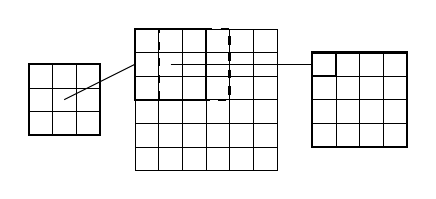
\begin{tikzpicture}[scale=0.30](18,3) 

\draw[thick] (0,1.5) rectangle (3, 4.5);
\draw[thick] (12, 1) rectangle (16, 5);
\draw[thick] (12, 4) rectangle (13, 5);

\draw[thick] (4.5, 3) rectangle (7.5, 6);
\draw[thick, dashed] (5.5, 3) rectangle (8.5, 6);

\draw[step=1, very thin, yshift=0.5cm] (0, 1) grid (3, 4);
\draw[step=1, very thin, xshift=0.5cm] (4, 0) grid (10, 6);
\draw[step=1, very thin] (12, 1) grid (16, 5);

\draw (1.5, 3) -- (4.5, 4.5);
\draw (6, 4.5) -- (12, 4.5);

\end{tikzpicture}
\caption{$\tilde{X_i}$ is the decoded output that resembles the input}
\label{fig:ae}
\end{figure}

\newpage

\subsubsection{Recurrent Neural Networks}
\label{recurrent}



\subsection{The Limitations of Machine Learning}
\label{limit}








